

\documentclass[11pt]{article}

\usepackage{amsmath,amsfonts,amssymb,enumitem}
\usepackage[]{graphicx}
\usepackage[usenames,dvipsnames]{xcolor}
\usepackage{colortbl}
\usepackage{wrapfig}
\usepackage{longtable}
\usepackage{tabularx}
\usepackage[version=3]{mhchem}
\usepackage[disable,colorinlistoftodos, color=blue!20!white, bordercolor=gray,
textsize=tiny,textwidth=1.0in]{todonotes}
\usepackage[final]{pdfpages}

\usepackage[font=footnotesize,format=plain,labelfont=bf]{caption}
\usepackage{multirow}
\usepackage{array}
\usepackage{booktabs}
\usepackage{pifont}
\usepackage{comment}
%\usepackage{overcite}

\usepackage{hyperref}
\hypersetup{hidelinks}
\usepackage{subfigure}
\usepackage{float}
\usepackage{pdflscape}
\usepackage{bm}
\usepackage{xfrac}
\usepackage{algorithm}
\usepackage{algpseudocode}

\usepackage[usestackEOL]{stackengine}


%%%%%%% CODES
\newcommand{\PlasComCM}{\textit{PlasComCM}}
\newcommand{\PlasComCMtwo}{\textit{PlasCom2}}
\newcommand{\goldenCopy}{\textit{golden copy}}
\newcommand{\GoldenCopy}{\textit{Golden Copy}}
\newcommand{\cl}[1]{\textit{codelet-#1}}
\newcommand{\Cl}[1]{\textit{Codelet-#1}}
\newcommand{\plusplus}[1]{#1{}\texttt{++}}
\newcommand{\ceesdcode}{\textit{MIRGE-Com}}
\newcommand{\ceesdMIRGE}{\textit{MIRGE}}
\newcommand{\ceesdbasiccode}{\textit{M-Com}}
\newcommand{\MIRGECom}{\textit{MIRGE-Com}}
\newcommand{\mirgecom}{\ceesdMIRGE}
\newcommand{\MIRGEHeat}{\textit{MIRGE-Heat}}
\newcommand{\ABaTe}{\textit{A\!Ba\!Te}}

\definecolor{tab-blue}{HTML}{1f77b4}
\definecolor{tab-orange}{HTML}{ff7f0e}
\definecolor{tab-green}{HTML}{2ca02c}
\definecolor{tab-red}{HTML}{d62728}
\definecolor{tab-purple}{HTML}{9467bd}
\definecolor{tab-brown}{HTML}{8c564b}
\definecolor{tab-pink}{HTML}{e377c2}
\definecolor{tab-gray}{HTML}{7f7f7f}
\definecolor{tab-olive}{HTML}{bcbd22}
\definecolor{tab-cyan}{HTML}{17becf}

\newcommand{\preqex}[1]{{\color{tab-purple} \textit{#1}}}
\newcommand{\preqcoop}[1]{{\color{tab-green} \textit{#1}}}
\newcommand{\preqceesd}[1]{{\color{tab-blue} \textit{#1}}}

\newcommand{\pop}[1]{{\color{tab-brown} \textit{#1}}}
\newcommand{\popceesd}[1]{{\color{tab-red} \textit{#1}}}

\newcommand{\pother}[1]{{\color{tab-orange} \textit{#1}}}

\newcommand{\clink}{{\tiny({\color{blue} link})}}

\newcommand{\Q}[1]{{\medskip\small\noindent\color{red}#1\par}}

%%%%%%% ANIMATIONS
\newcommand{\insertmovie}[3]{\ifmovies{
\movie[autostart,loop]
{\includegraphics[width=#1\textwidth]{Movies/#2}}
{Movies/#3}
}
\else{
\includegraphics[width=#1\textwidth]{Movies/#2}
}
\fi
}


%%%%%%%%% COLORS
\definecolor{RED}{RGB}{255,0,0}  %%%
\definecolor{myBlue}{RGB}{19,41,75}  %%% BLUE
\definecolor{myBlueLink}{RGB}{70,70,200}  %%% ILLINOIS BLUE
\definecolor{myOrange}{RGB}{232,74,39}   %%% ILLINOIS ORANGE
\definecolor{IllinoisOrange}{RGB}{232,74,39}  %%% ILLINOIS ORANGE
\definecolor{IllinoisBlue}{RGB}{19,41,75}   %%% ILLINOIS BLUE
\definecolor{mainTextColor}{RGB}{19,41,75}  %%% ILLINOIS BLUE
\definecolor{myLightGray}{rgb}{0.95,0.95,0.95}

\definecolor{ForestGreen}{rgb}{0.0, 0.2, 0.13}
\definecolor{darkpastelgreen}{rgb}{0.01, 0.75, 0.24}
\definecolor{antiquewhite}{rgb}{0.98, 0.92, 0.84}

\newcommand{\makeRed}[1]{{\color{red} #1}}
\newcommand{\makeBlue}[1]{{\color{blue} #1}}
\newcommand{\makeOrange}[1]{{\color{orange} #1}}
\newcommand{\makeGreen}[1]{{\color{ForestGreen} #1}}


%%%%%%%%% COMMENTS/INSTRUCTIONS/NOTES
\newcommand{\instr}[1]{{\newpage\thispagestyle{empty}\sf\color{red}INSTRUCTIONS:\color{blue}\\\bigskip\\#1\clearpage\newpage \setcounter{page}{1}}}
\newenvironment{notes}{\color{red}\footnotesize \begin{center}\begin{minipage}{0.8\textwidth}}{\end{minipage}\end{center}}
\newcommand{\CHK}{{\color{Red}CHK???}}
\newcommand{\CHKCS}{{\color{Green}CHK CS ???}}
\newcommand{\CHKWDG}{{\color{Green}CHK BILL ???}}
\newcommand{\CHKLNO}{{\color{Orange}CHK LUKE ???}}
\newcommand{\CHKAK}{{\color{Blue}CHK ANDREAS ???}}

%%%% DISABLE
\renewcommand{\CHK}{}
\renewcommand{\CHKCS}{}
\renewcommand{\CHKWDG}{}
\renewcommand{\CHKLNO}{}
\renewcommand{\CHKAK}{}


%%%%%%%%% FORMATTING
\captionsetup{labelfont={color=myOrange,bf},textfont={color=myBlue}}
\newcommand{\HRule}[2]{{\color{myOrange}\rule{#1}{#2}}}
\newcommand{\tPI}[1]{{\color{myOrange}#1}}
\newcommand{\ttPI}[1]{\texttt{\color{myOrange}#1}}
\newcommand{\sPI}[1]{\textsc{\color{myOrange}#1}}
\newcommand{\cPI}[1]{\textbf{\color{myOrange}#1}}
\newcommand{\rPI}[1]{\textrm{\color{myOrange}#1}}
\newcommand{\iPI}[1]{\textit{\color{myOrange}#1}}
\newcommand{\code}[1]{\textit{#1}}

\newcommand{\lead}[1]{\textit{\color{myOrange}(#1)}}
\newcommand{\tabtit}[1]{\textsc{\color{myOrange}#1}}
\newcommand{\entry}[1]{\mbox{\sffamily\bfseries{#1:}}\hfil}%
\newcommand{\bitem}{\item[{\color{myOrange}$\bullet$}]}
\newcommand{\oitem}{\item[{\color{myOrange}$\circ$}]}
\newcommand{\cditem}{\item[{\color{myOrange}$\cdot$}]}
\newcommand{\bmath}{\boldsymbol}
\newcommand{\eps}{\varepsilon}
\newcommand{\Dpartial}[2]{\frac{\partial #1}{\partial #2}}
\newcommand{\itemcolor}[1]{% Update list item colour
\renewcommand{\makelabel}[1]{\color{#1}\hfil ##1}}
\newcommand{\cM}{\mathcal{M}}
\newcommand{\gdotfill}{{\color{gray}\dotfill}}
\newcommand{\bvec}[1]{\ensuremath{\boldsymbol{#1}}}
\newcommand{\matrd}[1]{\ensuremath{\mathsf{#1}}}
\newcommand{\cmark}{\ding{51}}%
\newcommand{\xmark}{\ding{55}}%
%\newcommand{\parab}[2]{\vspace{#1 pt}\noindent \paragraph{\bf #2 \\}}

\newcommand{\mr}[1]{\multirow{2}{*}{#1}}
\newcommand{\mriii}[1]{\multirow{3}{*}{#1}}

\newcommand{\bbC}{\mathbb{C}}
\newcommand{\vbbm}{{\vec{m}}}
\newcommand{\bbM}{\mathbb{M}}
\newcommand{\bbH}{\mathbb{H}}
\newcommand{\bbG}{\mathbb{G}}
\newcommand{\bbV}{\mathbb{V}}

\newcommand{\vD}{{\vec D}}
\newcommand{\vhD}{{\hat{D}}}
\newcommand{\vg}{{\vec g}}
\newcommand{\vphi}{{\vec\phi}}
\newcommand{\vOmega}{{\vec\Omega}}

\newcommand{\vF}{{\vec{F}}}
\newcommand{\vf}{{\vec{f}}}
\newcommand{\vb}{{\vec{b}}}
\newcommand{\vq}{{\vec{q}}}
\newcommand{\vqs}{{\vec{q}^{\,\color{red}*}}}

\newcommand{\cJ}{\mathcal{J}}
\newcommand{\cG}{\mathcal{G}}
\newcommand{\cI}{\mathcal{I}}
\newcommand{\cP}{\mathcal{P}}
\newcommand{\cN}{\mathcal{N}}
\newcommand{\cC}{\mathcal{C}}
\newcommand{\cO}{\mathcal{O}}

\newcommand{\rstar}{{\color{red}*}}
\newcommand{\rchk}{{\color{red} \checkmark}}
\newcommand{\gchk}{{\color{green} \checkmark}}
\newcommand{\rbul}{{\color{red} $\bullet$}}
\newcommand{\pbul}{{\color{myOrange} $\bullet$}}
\newcommand{\ro}{{\color{red} $\circ$}}

\newcommand{\rhoi}[1][i]{\rho_{#1}}
\newcommand{\dt}[1][t]{\partial_{#1}}
\newcommand{\dx}[1][{\textrm{\bf x}}]{\boldsymbol \partial_{#1}}
\newcommand{\Vi}[1][i]{\mathcal{V}_{#1}}
\newcommand{\Mi}[1][\textswab{i}]{\mathcal{M}_{#1}}
\newcommand{\omegai}[1][i]{\dot{\omega}_{#1}}
\newcommand{\grav}{{\bf g}}
\newcommand{\Etot}{\mathcal{E}}

\newcommand{\mBG}{m_{\text{\tiny BG}}}
\newcommand{\nBG}{n_{\text{\tiny BG}}}
\newcommand{\nIp}{n_{\text{\tiny $I^+$}}}
\newcommand{\nIm}{n_{\text{\tiny $I^-$}}}


\newcommand{\bE}{{\mathbf{E}}}
\newcommand{\bI}{{\mathbf{I}}}
\newcommand{\bq}{{\mathbf{q}}}
\newcommand{\btau}{{\boldsymbol{\tau}}}

\newcommand{\bv}{{\bar{v}}}
\newcommand{\bepsilon}{{\bar{\epsilon}}}

\newcommand{\ST}{{S_{\text{\tiny T}}}}

\newcommand{\vu}{\vec{u}}
\newcommand{\vQ}{\vec{Q}}
\newcommand{\veta}{\vec{\eta}}

\newcommand{\TODO}[1]{{\color{pink} \tiny TODO: #1}}
\newcommand{\mtc}[1]{{\color{blue} \small MTC: #1}}
\newcommand{\tulio}[1]{{\color{orange} \small Tulio: #1}}
\newcommand{\mja}[1]{{\color{red} \small MJA: #1}}
\newcommand{\mynote}[1]{{\color{green} \tiny #1}}
\newcommand{\prj}[2]{{\color{gray} #1 [#2]}}

\newcommand{\myoul}[1]{\color{myOrange}\underline{\smash{\color{pdcolor1} #1}}\color{pdcolor1}}
\newcommand{\ccdot}{\color{myOrange}$\circ$\color{pdcolor1}\;}
\newcommand{\cc}[1]{\color{myOrange}#1\color{pdcolor1}{}}



% Grad, div, curl, etc.
\newcommand{\vdot}{\mathop{\mbox{\boldmath{$\cdot$}}}}
\newcommand{\vddot}{\mathop{\mbox{\textbf{:}}}}
\newcommand{\bnabla}{\mbox{\boldmath{$\nabla$}}}
\newcommand{\Lapl}{\nabla^2}
\newcommand{\hLapl}{\nabla^2_{\!\mathrm{h}}}
\newcommand{\pLapl}{\nabla^2_{\!\!\!\perp}}


\arrayrulecolor{myOrange}

%%%%%%%%% PAGE DIMENSIONS
\setlength{\oddsidemargin}{0.0in}
\setlength{\textwidth}{6.5in}
\setlength{\topmargin}{-0.4in}
\setlength{\footskip}{0.2in}
\setlength{\textheight}{9.4in}
\setlength{\headheight}{0.2in}
\setlength{\headsep}{0.0in}

%%%%%%%%%%% FLOAT MANAGEMENT
 \renewcommand{\topfraction}{0.9}
    \renewcommand{\bottomfraction}{0.8}
    \setcounter{topnumber}{2}
    \setcounter{bottomnumber}{2}
    \setcounter{totalnumber}{4}     % 2 may work better
    \setcounter{dbltopnumber}{2}    % for 2-column pages
    \renewcommand{\dbltopfraction}{0.9}	% fit big float above 2-col. text
    \renewcommand{\textfraction}{0.07}	% allow minimal text w. figs
    \renewcommand{\floatpagefraction}{0.7}	% require fuller float pages
    \renewcommand{\dblfloatpagefraction}{0.7}	% require fuller float pages

%%%%%%%%%% PARAGRAPHING
\setlength{\parindent}{0pt}
\setlength{\parskip}{1.ex}
\renewcommand{\baselinestretch}{0.95}


%%%%%%%%% SECTIONING STUFF
\makeatletter
\renewcommand{\section}{\@startsection
{section}%
{0}%
{0mm}%
{0.2\baselineskip}%
{0.1\baselineskip}%
{\normalfont\Large\bfseries\color{myOrange}}}%
\makeatother

\makeatletter
\renewcommand{\subsection}{\@startsection
{subsection}%
{1}%
{0mm}%
{0.3\baselineskip}%
{0.1\baselineskip}%
{\normalfont\large\bfseries\color{myOrange}}}%
\makeatother

\makeatletter
\renewcommand{\subsubsection}{\@startsection
{subsubsection}%
{1}%
{0mm}%
{0.1\baselineskip}%
{0.1\baselineskip}%
{\normalfont\normalsize\itshape\centering\color{myOrange}}}%
\makeatother


\renewcommand{\thesection}{\arabic{section}}
\renewcommand{\thesubsection}{\thesection.\arabic{subsection}}

\newcommand{\codebox}[1]{\vspace*{-0.15in}
\begin{center}
\fcolorbox{myOrange}{myLightGray}{
\begin{minipage}{0.96\textwidth}
\noindent\footnotesize
{#1}\par
\end{minipage}}
\end{center}
\vspace*{-0.15in}
}


\newcommand{\myhref}[2]{\href{#1}{{#2}}}

\newenvironment{noinditemize}
{\begin{itemize}[leftmargin=*,label=\color{myOrange}$\bullet$,itemsep=0in]\raggedright}
{\end{itemize}}

\newenvironment{tnoinditemize}
{\begin{tiny}\begin{noinditemize}}
{\end{noinditemize}\end{tiny}}


\usepackage{titleps,kantlipsum}
\newpagestyle{mypage}{%
  \sethead{}{}{}
  % \sethead{\raisebox{0.5in}{\tiny \color{myOrange}
  %     {\sectiontitle}}}{}
  % {\raisebox{0.5in}{\tiny \color{myOrange} \subsectiontitle}}
  \setfoot{}{\footnotesize\color{myOrange} \thepage}{}
}
\settitlemarks{section,subsection,subsubsection}
\pagestyle{mypage}



%%%%%%% INTERNSHIP STATUS
\newcommand{\MUST}{{\footnotesize\color{red} \textbf{MUST}}}
\newcommand{\WISH}{{\footnotesize\color{orange} \textbf{WISH}}}
\newcommand{\DEFER}{{\footnotesize\color{yellow} \textbf{DEFER}}}
\newcommand{\RETURN}{{\footnotesize\color{blue} \textbf{RETURN}}}
\newcommand{\DONE}{{\footnotesize\color{ForestGreen} \textbf{COMPLETED}}}
\newcommand{\PLAN}{{\footnotesize\color{green} \textbf{PLANNED}}}
\newcommand{\CURRENT}{{\footnotesize\color{cyan} \textbf{NOW}}}
\newcommand{\MAYBE}{{\footnotesize\color{lightgray} \textbf{MAYBE}}}

\newcommand{\SNL}{{\footnotesize $\;\rightarrow$ SNL}}
\newcommand{\LLNL}{{\footnotesize $\;\rightarrow$ LLNL}}
\newcommand{\LANL}{{\footnotesize $\;\rightarrow$ LANL}}


\newcommand{\aMUST}{\tiny\raisebox{1.5pt}{\color{red} (\textbf{M})}}
\newcommand{\aWISH}{\raisebox{1.5pt}{\tiny\color{orange} (\textbf{W})}}
\newcommand{\aDEFER}{\raisebox{1.5pt}{\tiny\color{yellow} (\textbf{D})}}
\newcommand{\aRETURN}{\raisebox{1.5pt}{\tiny\color{blue} (\textbf{R})}}
\newcommand{\aDONE}{\raisebox{1.5pt}{\tiny\color{ForestGreen} (\textbf{C})}}
\newcommand{\aPLAN}{\raisebox{1.5pt}{\tiny\color{green} (\textbf{P})}}
\newcommand{\aCURRENT}{\raisebox{1.5pt}{\tiny\color{cyan} (\textbf{N})}}
\newcommand{\aMAYBE}{\raisebox{1.5pt}{\tiny\color{lightgray} (\textbf{M})}}

\newcommand{\fut}{$^*$}
\newcommand{\pas}{$^\dag$}
\newcommand{\ant}{$^\ddag$}
\newcommand{\mat}{$^\S$}
\newcommand{\fel}{$^\circ$}


\renewcommand{\vec}[1]{\bm{#1}}

\usepackage{listings}

\definecolor{mintedlikecommentcolor}{rgb}{0.16,0.51,0.51}
\definecolor{mintedlikekeywordcolor}{rgb}{0,0.6,0}
\definecolor{mintedlikestringcolor}{rgb}{0.79,0,0}
\newcommand{\mintedlikebasicstyle}[1]{\ttfamily#1\linespread{4}}
\lstdefinestyle{mintedlike}{
    language=python,
    basicstyle=\mintedlikebasicstyle{\normalsize},
    commentstyle=\itshape\color{mintedlikecommentcolor},
    keywordstyle=\color{mintedlikekeywordcolor},
    stringstyle=\color{mintedlikestringcolor},
    columns=fullflexible,
    breakatwhitespace=false,
    breaklines=false,
    keepspaces=true,
    showspaces=false,
    showstringspaces=false,
    showtabs=false,
    tabsize=4,
    escapeinside=@@
}

%%%%%%%%%%%%%%%%%%%%%%%%%%%%%%%%%%%%%%%%%%%%%
\begin{document}
\color{mainTextColor}

\thispagestyle{empty}

\vspace*{1.0in}


\begin{center}

  {\Large \sPI{Internal CEESD Report}}\\

  \bigskip


  {\huge \cPI{\ceesdcode{} Performance Testing}}\\
  \bigskip

\bigskip

\rPI{M. Campbell}\\

\bigskip

  {\today}\\


\vspace*{1.0in}

\begin{minipage}{0.8\textwidth}
This report describes an effort to evaluate and model the computational performance of the Discontinuous Galerkin application \ceesdcode{}.
\end{minipage}

\end{center}
\vfill

\newpage
\setcounter{page}{1}

%\title{\textit{MIRGE-Com} Performance Testing}
%\author{}
%\date{}

%\begin{document}
%\maketitle

\section{Overview}
This is a working document used in a project to develop an Advection-Diffusion Transport (ADT) operator in \textit{MIRGE-Com}.  We will develop and evaluate a performance model for this operator, and evaluate the implementation against a few other codes. Some possible othe codes:
\begin{itemize}
\item \textit{DealII}
\item \textit{paranumal}
\item \textit{MFEM}
\item \textit{Nek5000}
\end{itemize}

\section{Model Problem}

The conservation system used for this performance study is the scalar (ADT).   This system is chosen because it features the major mathematical and computational components required of many systems of interest, including the Navier-Stokes equations. The ADT system admits an analytic solution, and is relatively easily modeled computationally.

The equations of ADT will be described in the following sections, along with an analytic solution. In the following, the scalar field $Q(\vec{x}, t)$ is transported through a medium with advective velocity $\vec{v}$ and diffusivity $D$; both are static, uniform parameters.

\subsection{Governing Equations}
In general, a scalar conservation law states that the time rate-of-change in the scalar field in a volume must be balanced by the ``flow'' of the scalar ``material'' across the volume boundary:   
\begin{equation}
  \frac{\partial Q}{\partial t} + \nabla \cdot \vec{F} = 0
  \label{eq:law}
\end{equation}

where $\vec{F}$ represents the total flux of the material. In the ADT system, the flux $\vec{F}$  consists of the advective and diffusive parts, $\vec{F}_{\text{adv}}$ and $\vec{F}_{\text{diff}}$, respectively:
\[
\vec{F} = \vec{F}_{\text{adv}} + \vec{F}_{\text{diff}}
\]

The advective flux, $\vec{F}_{\text{adv}}$, due to the motion of the medium at fixed, uniform velocity $\vec{v}$, is given by:
\[
\vec{F}_{\text{adv}} = Q\vec{v}
\]
The diffusive flux, $\vec{F}_{\text{diff}}$, is given by Fick's law:
\[
\vec{F}_{\text{diff}} = -D \nabla Q
\]

Substituting the expressions for the fluxes into Equation~\ref{eq:law} yields the following expression for the ADT system:
\begin{equation}
  \frac{\partial Q}{\partial t} + \nabla \cdot (Q\vec{v} - D \nabla Q) = 0
  \label{eq:adt}
\end{equation}

This represents the conservation of $Q$, where the change in $Q$ within a volume is balanced by the advective and diffusive fluxes across its boundary.

\subsection{Particular ADT Solution: Decaying Trig Function}
Consider a decaying scalar wave field of the form:
\begin{equation}
Q = A e^{-\alpha t} \cos\left(\vec{k} \cdot (\vec{x} - \vec{v} t)\right)
\end{equation}

where $A$, $\alpha$ are constants, $\vec{v}$ is the advection velocity, and $\vec{k}$ is the wave vector which specifies the orientation of the wave.

\subsubsection{Time derivative}

The time derivative of $Q$:
\[
\frac{\partial Q}{\partial t} = -\alpha Q + (\vec{k} \cdot \vec{v}) A e^{-\alpha t}\sin\left(\vec{k} \cdot (\vec{x} - \vec{v} t)\right)
\]
Making the following substitution:
\begin{equation}
 \omega=\vec{k}\cdot\vec{v}, \quad \tilde{Q} = A e^{-\alpha t}\sin\left((\vec{k} \cdot \vec{x}) - \omega t\right)
\end{equation}

the time derivative can be written more succinctly as:
\begin{equation}
  \frac{\partial Q}{\partial t} = \left(\omega \tilde{Q} - \alpha Q\right)
  \label{eq:dt}
\end{equation}


\subsubsection{Spatial derivatives}
The gradient:
\begin{equation}
  \nabla Q = -\vec{k}\tilde{Q}
  \label{eq:dx}
\end{equation}
The Laplacian:
\begin{equation}
  \nabla^2 Q = \nabla \cdot -\vec{k}\tilde{Q} = -|\vec{k}|^2 Q
  \label{eq:d2x}
\end{equation}

\subsubsection{Condition for balance}

Distributing the derivative operator in the ADT Equation~\ref{eq:adt} gives:
\[
\frac{\partial Q}{\partial t} + \nabla Q \cdot \vec{v} - D \nabla^2 Q = 0
\]

Substituting the derivative expressions from Equations~\ref{eq:dt}, \ref{eq:dx}, and \ref{eq:d2x} yields:
\[
\left(\omega \tilde{Q} - \alpha Q\right) - \omega \tilde{Q} + D|\vec{k}|^2 Q = 0
\]

Gathering terms:
\begin{equation}
  (D|\vec{k}|^2 - \alpha)Q = 0
  \label{eq:condition}
\end{equation}

The condition for balance is:
\begin{equation}
\begin{aligned}
\alpha & = D |\vec{k}|^2
\end{aligned}
\label{eq:bal}
\end{equation}

The condition for balance is to choose the rate of decay $\alpha$ according to Equation~\ref{eq:bal}.

\subsubsection{Final expression}

Finally, the exact analytic solution to the ADT system can be expressed as:

\begin{equation}
  Q(\vec{x}, t) = A e^{-D|\vec{k}|^2 t} \cos\left(\vec{k} \cdot (\vec{x} - \vec{v} t)\right)
  \label{eq:phi}
\end{equation}

where $A$ is an arbitary constant.  The main parameters setting the solution character are the diffusivity $D$, and the wave vector $\vec{k}$, and the character of the medium is set by velocity $\vec{v}$.  Typically, one would set the wavelength of the wave, $\lambda$, and a unit vector $\hat{\vec{k}}$ specifying the orientation of the wave. Then the wave vector is set as:

\begin{equation}
  \vec{k} = \frac{2\pi}{\lambda}\hat{\vec{k}}
\end{equation}

\section{DG Discretization}

% Adapt docs from https://mirgecom.readthedocs.io/en/latest/discretization.html

\ceesdcode{} currently employs a DG strategy akin to the \textit{BR1} algorithm outlined in
[Bassi\_1997], but with thermal terms and chemical reaction sources as outlined in
[Ihme\_2014] and [Cook\_2009].

\subsection{Recasting ADT for DG}

The ADT equations are rewritten as the following coupled system for two unknowns,
$\mathbf{Q}$, and $\mathbf{\Sigma}$.

\begin{align}
\mathbf{\Sigma} - \nabla{Q} &= \mathbf{0}\quad{\text{auxiliary eqn}}\\
\frac{\partial Q}{\partial t} + \underbrace{\nabla\cdot\mathbf{F}_\text{adv}(Q) -
\nabla\cdot\mathbf{F}_\text{diff}(Q,\mathbf{\Sigma})}_{= \nabla\cdot\mathbf{F}(Q,
\mathbf{\Sigma})} &= \mathbf{0} \quad{\text{primary eqn}}
\end{align}

At each time level, we first solve the auxiliary equation for the gradient of $Q, \vec{\Sigma}$, which is used to compute the diffusive fluxes $\vec{F}_\text{diff}$.  Then we solve the primary equation for the time rate of change of $Q$.

Let $\Omega_h$ denote a collection of disjoint elements $E$. The DG method constructs approximations $Q_h$, and $\mathbf{\Sigma}_h$, to $Q$, and $\mathbf{\Sigma}$ respectively, in discontinuous finite element spaces. Here, and in what follows, we use the subscript \textit{h} to denote discrete quantities. For any integer $k$, we define the following discontinuous spaces of piecewise (vector-valued) polynomial functions:

\begin{align}
\mathbf{V}^k_h &= \left\lbrace \mathbf{v} \in L^2(\Omega_h)^N:
\mathbf{v}|_E \in \lbrack P^k(E) \rbrack^N, \forall E \in \Omega_h
\right\rbrace, \\
\mathbf{W}^k_h &= \left\lbrace \mathbf{w} \in L^2(\Omega_h)^{N\times d}:
\mathbf{w}|_E \in \lbrack P^k(E) \rbrack^{N\times d}, \forall E \in \Omega_h
\right\rbrace,
\end{align}

where the number of equations $N = 1$, and $d$ is the spatial dimension. Here, $P^k(E)$ denotes a polynomial space on $E$ consisting of functions of degree $\leq k$. The DG formulation is obtained by multiplying by ``test functions'' $\mathbf{v}_h \in \mathbf{V}^k_h$, and $\mathbf{w}_h \in \mathbf{W}^k_h$ (one for each equation respectively) and integrating over each element. 

The resulting DG problem reads as follows: find $(Q_h,\mathbf{\Sigma}_h) \in \mathbf{V}^k_h \times \mathbf{W}^k_h$ such that $\forall(\mathbf{v}_h, \mathbf{w}_h) \in \mathbf{V}^k_h \times \mathbf{W}^k_h$, we have:

\begin{align}
\sum_{E\in\Omega_h} \left\lbrack \int_E \mathbf{v}_h\frac{\partial Q_h}
{\partial t} d\Omega + \oint_{\partial E} \mathbf{v}_h h d\sigma - \int_E \nabla
\mathbf{v}_h\cdot\mathbf{F}(Q_h, \mathbf{\Sigma}_h)d\Omega\right\rbrack &= 0 \\
\sum_{E\in\Omega_h}\left\lbrack \int_E \mathbf{w}_h\mathbf{\Sigma}_h d\Omega -
\oint_{\partial E} \mathbf{w}_h\mathbf{H}_s d\sigma + \int_E \nabla\mathbf{w}_h Q_h d\Omega\right\rbrack &= 0,
\end{align}

where $h = h_a - h_d$ is a composite \textit{numerical flux} respectively representing the advective and diffusive contributions to the physical flux $\left(\mathbf{F}_\text{adv}(Q_h) - \mathbf{F}_\text{diff}(Q_h, \mathbf{\Sigma}_h\right)\cdot\mathbf{n}$, with $\mathbf{n}$ being the outward facing unit normal with respect to the local element. $\mathbf{H}_s$ is the \textit{gradient numerical flux} ($Q_h\mathbf{n}$) for the auxiliary equation. More details on the numerical fluxes are provided in the next section.

Since $\mathbf{F}_\text{adv}(Q_h)\cdot\mathbf{n}$ is discontinuous, the quantities are allowed to vary on either side of a shared element boundary. That is, $\mathbf{F}_\text{adv}(Q^+_h)\cdot\mathbf{n}^+ \neq \mathbf{F}_\text{adv}(Q^-_h)\cdot\mathbf{n}^-$. Here, $\mathbf{n}^+$ and $\mathbf{n}^-$ denote the ''cell-local'' (outward pointing) unit normals for elements $E^+$ and $E^-$ (respectively) which share a face: $\partial E^+ \cap \partial E^- \neq \emptyset$. Similarly for the diffusive and auxiliary fluxes $\mathbf{F}_\text{diff}(Q_h, \mathbf{\Sigma}_h)\cdot\mathbf{n}$, and $Q_h\mathbf{n}$.

Expanding out the trial and test functions (component-wise) in terms of the local element basis in each element:
\begin{align}
Q(\mathbf{x}, t)_h|_E = \sum_{i=1}^n Q_i(t)\phi_i^k(\mathbf{x}), \quad
\mathbf{\Sigma}(\mathbf{x})_h|_E = \sum_{i=1}^n \mathbf{\Sigma}_i\phi_i^k(\mathbf{x}),\\
\mathbf{v}(\mathbf{x})_h|_E = \sum_{i=1}^n \mathbf{v}_i\phi_i^k(\mathbf{x}), \quad
\mathbf{w}(\mathbf{x})_h|_E = \sum_{i=1}^n \mathbf{w}_i\phi_i^k(\mathbf{x}),\quad
\end{align}
allows us to obtain a set of algebraic equations for the conserved state $Q_h$ and the auxiliary gradient variable $\mathbf{\Sigma}_h$. That is, for each $j = 1, \dots, \dim P^k$, we have:
\begin{align}
\frac{d}{dt} \sum_{E\in\Omega_h}\int_E \phi_j^k Q_h d\Omega &= \sum_{E\in\Omega_h}
\left\lbrack\int_E \nabla\phi_j^k\cdot\left(\mathbf{F}_\text{diff}(Q_h, \mathbf{\Sigma}_h) -
\mathbf{F}_\text{adv}(Q_h)\right)d\Omega\right\rbrack \nonumber \\
&- \sum_{E\in\Omega_h}\left\lbrack\oint_{\partial E}\phi_j^k h_a(Q_h^\pm; \mathbf{n}) d\sigma + \oint_{\partial E} \phi_j^k h_d(Q_h^\pm,\mathbf{\Sigma}_h^\pm; \mathbf{n}) d\sigma\right\rbrack, \\
\sum_{E\in\Omega_h}\int_E\phi_j^k \mathbf{\Sigma}_h d\Omega &= \sum_{E\in\Omega_h}\left\lbrack
\oint_{\partial{E}}\phi_j^k \mathbf{H}_s(Q^\pm_h; \mathbf{n}
)d\sigma -
\int_E\nabla\phi^k_j Q_h d\Omega\right\rbrack. \\
\end{align}

With the aid of the DG element-local mass and stiffness operators are defined as:

\begin{align}
  \mathcal{M}_{ij} = \int_{E_h} \phi_i \phi_j dV,\quad \mathcal{S}_{ij} = \int_{E_h} \phi_i \nabla{\phi_j} dV, \quad \mathcal{M}^f_{ij} = \int_{\partial E_h} \hat{\phi}_i \hat{\phi}_j dS,\\
\end{align}

where $\hat{\phi}$ are the shape functions $\phi$ restricted to the element boundary $\partial E_h$, we can express the system as:

\begin{align}
\sum_{E\in\Omega_h} \mathcal{M} \dot{Q}_h &= \sum_{E\in\Omega_h}\left(
\mathcal{S} \mathbf{F}(Q_h, \mathbf{\Sigma}_h) - \mathcal{M}^f h(Q_h^\pm,\mathbf{\Sigma}_h^\pm; \mathbf{n}) \right),\\
\sum_{E\in\Omega_h} \mathcal{M} \mathbf{\Sigma}_h &= \sum_{E\in\Omega_h} \left( \mathcal{M}^f \mathbf{H}_s(Q^\pm_h; \mathbf{n}) - \mathcal{S} Q_h \right),
\end{align}

and the element-local expression for the primary and auxilliary equations:

\begin{align}
  \dot{Q}_h &= \mathcal{M}^{-1}\left(\mathcal{S} \mathbf{F} - \mathcal{M}^f h \right),\\
  \mathbf{\Sigma}_h &= \mathcal{M}^{-1}\left( \mathcal{M}^f \mathbf{H}_s - \mathcal{S} Q_h \right)
  \label{eq:algebraic}
\end{align}

The DG operators $\mathcal{M}, \mathcal{S}, and \mathcal{M}^f$ are provided by the \ceesdcode{} infrastructure, so we must express the ADT-specific constructs $Q, \mathbf{F} = \mathbf{F}_\text{diff} - \mathbf{F}_\text{adv}, h$ and $\mathbf{H}_s$ to advance the ADT system in \ceesdcode{}.

\subsection{Numerical fluxes}

Numerical fluxes are responsible for calculating the fluxes at all \textit{internal} DG element
boundaries, and are also sometimes used to transmit boundary conditions into the domain at the
domain boundary. Numerical fluxes must account for the discontinuities at element faces, and calculate
a single valued flux that both elements agree on.  That is, they must be functions
of both $\pm$ states, and must produce a consistent flux.

For a conservation law $\frac{\partial Q}{\partial t} + \nabla \cdot \mathbf{F}(Q) = \mathbf{S}$,
the numerical flux $h$ must satisfy the consistency relations

\begin{align}
   h(Q^+, Q^-; \mathbf{n}) &= \mathbf{F}(Q)\cdot\mathbf{n}  \\
   h(Q^+,Q^-;\mathbf{n}) &= -h(Q^-, Q^+;-\mathbf{n})
\end{align}

Specifically, for our system of equations, we use numerical flux functions $h_a$ for the
advective fluxes, $h_d$ for the diffusive fluxes, and $H_s$ for the gradient fluxes used in the
auxiliary equation.  More details on each of these numerical fluxes is provided in the following
sections.

\subsubsection{Numerical flux for advective terms}

In this performance-oriented study, where we have fixed velocity $\vec{v}$ and transport only smooth
$\mathcal{C}_\infty$ functions in $Q$, we choose simple central numerical fluxes for both the advective
and diffusive terms.

The central numerical flux for the divergence of the advective transport flux is implemented as:
\begin{align}
  h_{a}(Q_h^+, Q^-_h; \mathbf{n}) = \frac{1}{2}
  \left(\mathbf{F}_\text{adv}(Q_h^+)+\mathbf{F}_\text{adv}(Q_h^-)\right) \cdot \mathbf{n},
\end{align}


\subsubsection{Numerical Fluxes for diffusive terms}

The numerical flux function used for the divergence of the diffusive transport flux is implemented
as follows:

\begin{align}
   h_d(Q_h^+, \mathbf{\Sigma}_h^+, Q_h^-, \mathbf{\Sigma}_h^-;
   \mathbf{n}) = \frac{1}{2}\left(\mathbf{F}_\text{diff}^+ + \mathbf{F}_\text{diff}^-\right) \cdot \mathbf{n},
\end{align}

where $\mathbf{F}_\text{diff}^{\pm} \equiv \mathbf{F}_\text{diff}(Q_h^{\pm}, \mathbf{\Sigma}_h^{\pm})$, is the diffusive
flux function computed for the ($\pm$) sides of the element boundary, respectively.


\subsubsection{Numerical fluxes for the auxiliary equations (gradients)}

The numerical flux function used for the auxiliary equations (i.e. when computing the gradient
of the fluid solution and temperature) is implemented as follows:

\begin{align}
   \mathbf{H}_s(Q_h^+, Q_h^- ; \mathbf{n}) &= \frac{1}{2}\left(
   (Q_h^+ + Q_h^-)\right)\mathbf{n}
\end{align}

\section{Simulation Setup \& Configuration}

Configuration parameters:
\begin{itemize}
\item $\lambda$: solution wavelength
\item $\hat{\vec{k}}$: solution orientation
\item $\vec{v}$: advective velocity (arbitrary)
\item $N_{\text{el}}$: number of elements per axis
\end{itemize}

The remaining parameters are set as follows:
\begin{itemize}
  \item simulation timestep: $\Delta t = \frac{\lambda}{\sqrt{2} N_{\text{el}} |\vec{v}|}$
\end{itemize}
\subsection{Domain}

\begin{figure}[H]
  \begin{center}
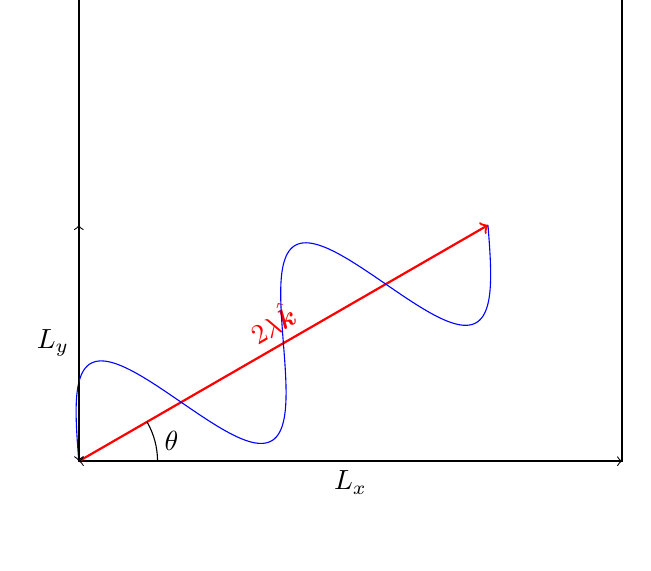
\begin{tikzpicture}

% Draw the box
\draw[thick] (0,0) rectangle (6.9,6);

% Draw the wave vector
\draw[->, thick, red] (0,0) -- (5.2, 3) node[midway, above, sloped] {$2\lambda\hat{\vec{k}}$};

% Define the wave parameters
\def\k{1}
\def\anga{30}

% Convert theta to radians for calculations
\pgfmathsetmacro{\thetarad}{\anga * pi / 180}

% Draw the wave aligned with the wave vector
\begin{scope}[rotate around={\anga:(0,0)}]
    \draw[blue, domain=0:6, samples=200] plot (\x, {sin(360 * \x / 3)});
\end{scope}

% Draw angles and dimensions
\draw[<->] (0,0) -- (6.9,0) node[midway, below] {$L_x$};
\draw[<->] (0,0) -- (0,3) node[midway, left] {$L_y$};

% Label the wave vector angle
\draw (1,0) arc[start angle=0,end angle=30,radius=1] node[midway, right] {$\theta$};

\end{tikzpicture}
\caption {2D domain example with wave orientation $\hat{\vec{k}}$, wavelength $\lambda$, and side lengths $[L_x, L_y] = [\frac{2\lambda}{\hat{\vec{k}}\cdot\hat{\vec{x}}}, \frac{\lambda}{\hat{\vec{k}}\cdot\hat{\vec{y}}}]$}
\end{center}
\end{figure}


\subsection{Initialization}

% No boundary conditions - periodic
% \subsection{Boundary Conditions}

\subsection{Simulation Parameters \& Resource Configuration}

\subsubsection{Domain decomposition}

\subsubsection{Partition-to-processor parameters}

\section{Performance Model}
\subsection{Formulation}
Write out the matrix/operator form of system equations in more detail, for use in the performance model.
\begin{align}
  \dot{Q} &= \mathbb{M}^{-1}\left(\mathbb{S}_{\hat{x}} F_x + \mathbb{S}_{\hat{y}} F_y + \mathbb{S}_{\hat{z}} F_z + \sum_\text{faces} \mathbb{M}_f h\right) \\
  \mathbf{\Sigma} &= \mathbb{M}^{-1}\left(\sum_{\text{faces}}{\mathbb{M}_f Q_h\hat{\mathbf{n}}} - <\mathbb{S}_{\hat{x}} Q, \mathbb{S}_{\hat{y}}Q, \mathbb{S}_{\hat{z}}Q>\right)
\end{align}
\subsection{DOF Counting}
Explain how to calculate the sizes of the DG operators.  How many DOFs per element of a given order? $\frac{\text{ndof}}{\text{element}}=\frac{(p+\text{dim})!}{(p!)(\text{dim}!)}$.

For example, a $p=1$ tetrahedral element will have $\frac{4!}{3!}$ DOFs, and its faces will each have $\frac{3!}{2!}$ DOFs.

\subsection{Algorithm}
Write a pseudo-code explanation of every step, especially those steps that are expected to impact performance.  The operators, assumed to be pre-caculated and provided my mirgecom are
\begin{itemize}
\item $\mathbb{M}$: Mass operator, $\text{ndof}_\text{el} \times \text{ndof}_\text{el}$
\item $\mathbb{M}^{-1}$: Inverse mass operator
\item $\mathbb{P}$: Projection operator $\text{ndof}_\text{face} \times \text{ndof}_\text{el}$
\item $\mathbb{S}_j$: Stiffness operator $\text{ndof}_\text{el} \times \text{ndof}_\text{el}$
\end{itemize}

A rough outline of the RHS algorithm for each element goes like this:
\begin{itemize}
\item project $Q$ to element faces (and communicate)  Example count: For each face we need a MatVec $\mathbb{P}(Q)$, which means we'll have nfaces*(ndof\_element X ndof\_element) (or something like that)
\item for n = 1 to $\frac{nfaces}{element}$
  \begin{itemize}
  \item compute gradient numerical flux for face $\mathbf{H}_f = \{\{Q\}\}\hat{\mathbf{n}}$ Example count, looking back at grad flux computation I count (4FLOPS / 6 LoadStores).
  \item $\mathbb{M}_f$ on each component (ndim * MatVec)
  \item accumulate to $\mathbf{H}$ (nfaces * FLOPS)
  \end{itemize}
\item $\vec{dQ} = \mathbb{S}_i Q$ (per dimension)
\item $\mathbb{M}^{-1}(\vec{dQ} + \mathbf{H})$ for $\nabla{Q}$
\item project $\nabla{Q}$ to element faces (and communicate)
\item compute advective flux $\mathbf{F}_\text{adv} = Q\vec{v}$
\item compute diffusive flux $\mathbf{F}_\text{diff} = -D\nabla{Q}$
 \item $\mathbf{F} = \left(\mathbf{F}_\text{adv} + mathbf{F}_\text{diff}\right)$ 
\item for n = 1 to $\frac{nfaces}{element}$
  \begin{itemize}
  \item compute advective flux $\mathbf{F}_\text{adv} = Q\vec{v}$
  \item compute diffusive flux $\mathbf{F}_\text{diff} = -D\nabla{Q}$
  \item $\mathbf{F} = \mathbf{F}_\text{diff} - \mathbf{F}_\text{adv}$
  \item compute numerical flux $h_f=\{\{\mathbf{F}\}\} \cdot \hat{\mathbf{n}}$
  \item compute facial contribution $\mathbb{M}_f h$
  \item accumulate to $h$
  \end{itemize}
\item $\nabla \cdot \mathbf{F} = \mathbb{S}_{\hat{x}}\mathbf{F}_x + \mathbb{S}_{\hat{y}}\mathbf{F}_y + \mathbb{S}_{\hat{z}}\mathbf{F_z}$
\item $\mathbb{M}^{-1}(h + \nabla\cdot\mathbf{F})$ for $\dot{Q}$
\end{itemize}

\begin{algorithm}
\caption{Compute RHS for Advection-Diffusion Equation using Discontinuous Galerkin Solver}
\begin{algorithmic}[1]
\State \textbf{Input:} $Q$, $\vec{v}$, $D$
\State \textbf{Output:} $\dot{Q}$
% \State Project $Q$ to element faces:
\For{each interior boundary $b_i$}
\State $\mathbb{P}(Q)$ ($\times \text{nfaces}_{b_i}$)
\If{$b_i$ is partition}
\State Exchange $Q$ across $b_i$, ($\text{nface}_{b_i} \times \text{ndof}_\text{face}$) values to communicate
\EndIf
\EndFor
%\For{each face $f$}
%  \State Compute $\mathbb{P}(Q)$ on $f$ \Comment{MatVec $\mathbb{P}(Q)$}
%\EndFor

\For{$n = 1$ to $\frac{nfaces}{element}$}
  \State Compute gradient numerical flux $\mathbf{H}_f = \{\{Q\}\}\hat{\mathbf{n}}$
  \State Apply $\mathbb{M}_f$ on each component
  \State Accumulate to $\mathbf{H}$
\EndFor

\State Compute $\vec{dQ} = \mathbb{S}_i Q$ (per dimension)
\State Compute $\nabla{Q} = \mathbb{M}^{-1}(\vec{dQ} + \mathbf{H})$

\State Project $\nabla{Q}$ to element faces (and communicate)
\State Compute advective flux $\mathbf{F}_\text{adv} = Q\vec{v}$
\State Compute diffusive flux $\mathbf{F}_\text{diff} = -D\nabla{Q}$
\State $\mathbf{F} = \mathbf{F}_\text{adv} + \mathbf{F}_\text{diff}$

\For{$n = 1$ to $\frac{nfaces}{element}$}
  \State Compute advective flux $\mathbf{F}_\text{adv} = Q\vec{v}$
  \State Compute diffusive flux $\mathbf{F}_\text{diff} = -D\nabla{Q}$
  \State $\mathbf{F} = \mathbf{F}_\text{diff} - \mathbf{F}_\text{adv}$
  \State Compute numerical flux $h_f=\{\{\mathbf{F}\}\} \cdot \hat{\mathbf{n}}$
  \State Compute facial contribution $\mathbb{M}_f h$
  \State Accumulate to $h$
\EndFor

\State Compute $\nabla \cdot \mathbf{F} = \mathbb{S}_{\hat{x}}\mathbf{F}_x + \mathbb{S}_{\hat{y}}\mathbf{F}_y + \mathbb{S}_{\hat{z}}\mathbf{F}_z$
\State Compute $\dot{Q} = \mathbb{M}^{-1}(h + \nabla \cdot \mathbf{F})$
\end{algorithmic}
\end{algorithm}

\subsection{Expected performance}
\subsubsection{General operators}
What FLOPs, memory requirements do we expect for MatMat, MatVec, scalar operations appearing in the DG code.
\subsubsection{ADT system}
Based on the previous two sections, write out the expected performance of each component.  Make a count of the
components and for each, include:
\begin{itemize}
\item Number of FLOPs
\item Memory Load-and-Stores
\end{itemize}

\section{Numerical Results}
\subsection{ADT}
\subsection{Performance}

\end{document}
